\chapter{Sensoristica}
Esistono diverse tipologie di sensori per acquisire dati.

\section{Sensori a stato solido}
I sensori a stato solido sono quelli presenti nelle telecamere e si dicono a stato 
solido perché le componenti sono ferme, non in movimento. 

\subsection{CCD}
I primi sensori si basavano 
sui \textbf{CCD} ovvero registri a scorrimento, il modello vienme rappresentanto 
nella figura \ref{fig:modello_sensori_stato_solido}.

\begin{figure}[h]
    \centering
    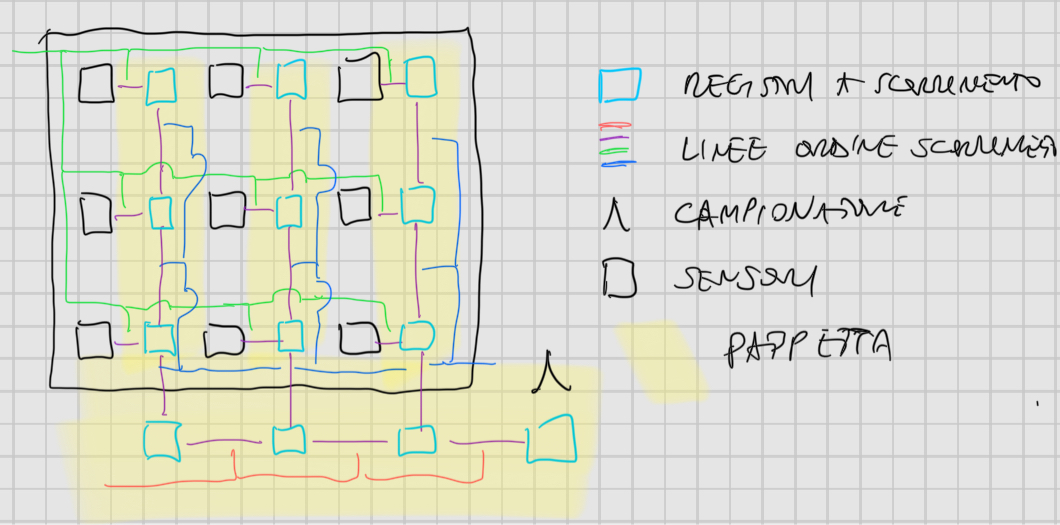
\includegraphics[width=0.5 \textwidth]{figure/modello_sensori_solidi.jpg}
    \caption{Modello dei sensori a stato solido}
    \label{fig:modello_sensori_stato_solido}
\end{figure}

Si ha la matrice di componenti sensibili collegate direttamente a delle celle dei 
registri di scorrimento coperte da una pappetta che evita la sovrascrizione dei 
registri da parte dell'energia. I registri sono collegati con gli elementi sensibili 
e anche tra di loro permettendo di acquisire l'immagine e digitalizzarla. Il 
processo di acquisizione dell'immagine è il seguente:
\begin{enumerate}
    \item entra l'energia nel sensore che viene assorbita dagli elementi sensibili.
    \item si abilita l'ordine di scorrimento, linea verde, (abilita l'interruttore) dagli elementi 
    sensibili alle celle dei registri direttamente connesse. Questo passaggio è
    una trasmissione e causa una perdita di energia però questo permette il suo 
    salvataggio nel registro. In questo modo gli elementi sensibili sono stati 
    svuotati, si disconnettono gli elementi dalle celle e in questo modo tornato 
    ad acquisire la nuova luce.
    \item si attivano le line blu per far scorrere l'energia verso il basso riempiendo 
    la linea di registri inferiore
    \item si attivano le linee rosse per scorrere a destra l'energia che viene 
    catturata e digitalizzata da un campionatore. Questo corrisponde a digitalizzare 
    un singolo pixel alla volta. Si ripete questo punto per il numero di colonne
    in modo da digitalizzare una riga e poi si ripete dal punto $3$ per salvare 
    mano a mano tutte le righe di pixel. 
\end{enumerate} 

Al posto di un campionatore posso ottenere un segnale \textbf{video composito} 
rappresentante la riga e verrà campionata un'asta alla volta del segnale video coposito.
Questa architettura basata su un elemento sensibile connesso ad un elemento 
nascosto differente viene chiamata \textbf{interline transfert CCD}.

Il problema di questo approccio è che si perde l'energia che si scontra contro la 
pappetta quindi si abbassa la qualità e la luminosità dell'immagine. Quindi molto 
spesso si aggiungono delle \textbf{microlenti} sopra alla pappetta per riflettere 
il segnale verso l'elemento sensibile più vicino e questo permette di aumentare la 
qualità dell'immagine quando si ha poca luce.

Un altro problema di questo modello è che si possono avere dei rumori dovuti al 
surriscaldamento del sensore, questo è dovuto dallo spostamento di energia nei 
vari registri che si può perdere trasformandosi in calore, rischiando di aggiungere 
del rumore agli elementi sensibili. Per risolverlo si può raffreddare il sensore.

L'utilizzo del segnale video composito sta scomparendo, generalmente viene utilizzato 
nelle camere di fascia bassa per contenere i costi del dispositivo. Da notare che 
spesso è utile anche perché permette di trasferire il segnare verso la regione 
della macchina fotografica adibita a elaborazione che prima digitalizzerà il segnale.

Per risparmiare sulla costruzione si utilizza il video composito nelle metodologie 
a \textbf{scansione interlacciata} dove si ha 1 elemento nascosto direttamente connesso
a due elementi sensibili su due righe differenti. In sostanza l'acquisizione avviene 
in due tempi, prima le righe pari e poi le righe dispari della camera. Questo porta 
anche alla formazione di artefatti nell'immagine.

Un altra tecnica per risparmiare è il modello \textbf{interlacciato CCD} che è come 
il CCD ma con la metà delle righe, quindi si ha una risoluzione dimezzata.

Un'altra architettura simile al CCD è il \textbf{frame trasfert CCD} dove sulla parte 
del sensore si hanno solo elementi sensibili collegati ai registri a scorrimento 
al di fuori del sensore. Questo permette di essere più fitti perché c'è bisogno solo 
di lasciare lo spazio per le linee e quindi ci possono stare più elementi sensibili.

I sensori a stato solido hanno anche una \textbf{efficienza quantistica particolare}
infatti il picco di frequenze di energia che percepiscono è più spostato nel NIR
rispetto all'occhio umano, questo significa che fanno più fatica a \textbf{trasdurre}
in carica le frequenze più vicine al blu piuttosto quelle che più vicine al rosso.
Questo significa che ci si allontana dalla fedeltà cromatica.

Quando lavoriamo con ottiche per NIR e per il visibile, dobbiamo sottolineare 
che hanno \textbf{indici di rifrazione differenti} in base alla lunghezza dell'onda e quindi 
possiamo avere diversi comportamenti sul fuoco per frequenze nel visibile e frequenze NIR.

\subsection{CMOS}
Per i sensori a stato solido posso avere anche un'altra architettura basata sull'\textbf{indirizzamento
diretto} dei singoli elementi sensibili (CMOS). Più precismante si ha sempre una matrice 
di elementi sensibili nel sensore, in aggiunta si ha una circuiteria che permette 
l'indirizzamento diretto di un pixel per portarlo sulla pista di output per scaricare 
l'elemento sensibile. Sulla pista di output possiamo avere un digitalizzatore o 
un convertitore per ottenere un segnale già digitale.

Per quanto riguarda il diagramma di \textbf{efficienza quantistica} delle CMOS si ha una 
decrescita più blanda della camera nella sensibilità verso le frequenze NIR quindi 
sono più adatte alla visione notturna rispetto alle CCD.

Per avere maggior sensibilità sulle frequenze MIR e LIR non si utilizzano 
CMOS e CCD ma altri conduttori non basati sul silicio.

\subsection{Tempo di esposizione e blur}
Il \textbf{tempo di esposizione} del sensore nella fotografia (tempo di integrazione 
dell'energia incidente) è l'intervallo di tempo di conversione da energia incidente 
e conversione in segnale. In sostanza è il tempo che intercorre tra due letture,
questa tempistica deve essere massima con poca luce o minima per scene dinamiche 
altrimenti otteniamo il motion blur.
\begin{nota}
    Abbiamo due tipologie di blur:
    \begin{itemize}
        \item \textbf{circle blur}: quando la scena è statica allora lo sfocamento 
        è dato dall'apparato
        \item \textbf{motion blur}: quando la scena è dinamica e la sfocatura è data 
        dal fatto che si hanno punti che si spostano tra i pixel quindi verranno proiettati 
        su più pixel in base al movimento
    \end{itemize}

    Da notare che il motion blur non si vede quando l'oggetto si muove lungo l'asse 
    di proiezione ed è lontano.
\end{nota}

\subsection{Rolling shutter e global shutter}
Dato un tempo di esposizione, per le macchine basate su indirizzamento diretto 
possono avere un'acquisizione a \textbf{rolling shutter} ovvero un'acquisizione 
delle singole componenti sensibili ad intervalli differenti comportando un tempo 
di esposizione per ogni singolo elemento sensibile differente da tutti gli altri.
Questo può essere un problema quando siamo in computer vision e quando abbiamo 
un ampio tempo di acquisizione e una scena dinamica. Se abbiamo \textbf{rolling shutter}
esposizione molto bassa allora l'effetto potrebbe essere trascurabile. 
Il contrario al \textbf{global shutter} significa che l'acquisizione delle singole 
componenti sensibili è uguale per tutti gli elementi e questo lo otteniamo di default dalle 
camere CCD, invece in un sistema CMOS bisogna complicare il modello e non è semplice. 

\begin{nota}
    Le rolling shutter possono essere utili magari quando hanno una alta sensibilità
\end{nota}


\subsection{Blooming/snearing per sensori a stato solido}

Questi sensori rispetto ai sensori a tubo hanno una relazione tra energia incidente 
e conversione in segnale analogico lineare fino alla saturazione. La parte in cui 
si satura genera dei problemi come il \textbf{blooming/snearing}.
Quando si arriva a saturazione e continua 
ad entrare energia allora genera degli aumenti di luce in zone in cui non ci 
sarebbero. Un esempio è quando inquadriamo il sole e non vediamo un cerchio 
chiaro ma vediamo un romboide di luce. La forma risultante dipende da come è 
fatto il sensore, in generale si espande la luce in base alla vicinanza delle 
zone sensibili ex: elementi sulla stessa colonna. Per risolvere questo problema 
possiamo aggiungere degli elementi isolanti tra gli elementi sensibili che assorbono
l'espansione della luce, in ogni caso c'è meno spazio tra elementi sensoriali
sulle colonne ridotto e quindi si espande la luce.



\subsection{Sensori HDR}
Le CMOS sono buone lato consuming perché sono economiche, ma lato cv no per
la questione del rolling shutter e le diverse esposizioni. Per noi possono essere
utili per il problema del \textbf{High Dynamic Range} dove per dinamica si intende 
la dinamica del dato analogico che esce da ciascun elemento sensibile. In sostanza 
il delta tra massima luce e massima oscurità non è comparabile con quello umano,
per simularlo in fotografia si scattano una serie di foto a diversi tempi di esposizione 
e poi si uniscono queste foto con un algoritmo per ottenerne una HDR. In CV noi possiamo 
utilizzare CMOS per aggiungere circuiteria sui singoli pixel per implementare una 
sorta di HDR, ovviamente non sarà mai comparabile all'umano e a quello dei fotografi.
Esistono telecamere HDR di due tipologie:
\begin{itemize}
    \item \textbf{doppia esposizione}: ogni immagine è ottenuta da un mixture di 
    due immagini ad esposizione diversa, il problema è che la scena deve essere statica
    \item \textbf{CMOS-based}: sfruttano CMOS per aggiungere su ogni pixel un sistema che misura 
    la carica incidente, nel momento che raggiunge una soglia allora incrementa 
    il contantore, scarica l'elemento, si ricarica l'elemento con la luce e si 
    riesegue il ciclo in modo da ottenere livelli maggiori di lucentezza. Dati 
    sensori che vanno da 50-60 db mentre questi metodi arrivano a 110-120 db (ampiezza di range).
\end{itemize}

\subsection{Sensori 3D}
Sempre basate su CMOS sono le camere $3D$ basate sul principio del \textbf{tempo di volo} (ToF). 
In sostanza si ha un flash che fa partire 
un array bidimensionare di contatori (uno per ogni pixel) che misurano il tempo 
di rimbalzo della luce dall'emissione del flash alla ricezione degli elementi 
sensibili. Per avere una buona approsimazione della distanza si conta ad alta frequenza
e funzionano bene sotto i 10 metri, perché più andiamo lontani e meno luce torna 
al sensore.

Esistono altri approcci come Kinect che effettua una triangolazione con 2 camere,
un esempio di quelle basate sul tempo di volo sono i LIDAR.

\subsection{Camere a colori}
Esistono 2 modi per ottenere una immagine a colori: 3 sensori (3-CCD) che sono sensibili 
al rosso, verde, blu oppure l'approcio Bayer Filter. Il primo è più costoso

L'approccio per creare camere a colori è quello di usare il Bayer Filter, ovvero 
si prende la matrice dei pixel la si suddivide in blocchi di 2x2 di elementi sensitivi.
Ogni blocco avrà $2$ elementi sensibili al verde, uno al rosso e uno al blu, questo 
viene realizzato mediante l'applicazione di una pappetta che filtra solo quelle frequenze.
L'informazione $RGB$ è fornita per ciascuno dei blocchi e questo viene implementato 
mediante delle interpolazioni dei valori tra blocchi vicini, quindi ferequenze vicino 
al rosso e al blu hanno risoluzione $1/4$. Questo non è un problema lato consumer
perché non abbiamo ce ne accorgiamo a livello cromatico, infatti ci sono standard
che separano la comaticità e l'intensità in modo da sottocampionare la crominanza.
Il problema è che in CV abbiamo un problema perché hanno meno risoluzione rispetto 
a camere che hanno 3 sensori diverse, inoltre in fase di interpolazione si vedono 
pixel che non centrano nulla con il colore creando rumore fastidioso. Quindi le camere per CV professionali 
che usano il Bayer filter spesso implementano la possibilità di ottenere direttamente 
i valori non interpolati, lasciando all'utente la scelta dell'interpolazione. 

Un altro modo per implementare le camere a colori è quello di avere i sensori stackati 
uno sull'altro in modo tale da far si che le frequenze del B si fermano sul primo 
sensore, il G si fermano sul secondo e infine il R si fermano sull'ultimo. Questo 
permette di avere lo stesso effetto dei sensori a 3-CCD ma di non avere il costo 
e la loro fragilità, permettendoci quindi di avere un unico sensore che riconosce
le singole componenti RGB per ogni elemento sensitivo.
